\documentclass[12pt]{article}
\usepackage[a4paper]{geometry}
\usepackage[myheadings]{fullpage}
\usepackage{fancyhdr}
\usepackage{lastpage}
\usepackage{graphicx, wrapfig, subcaption, setspace, booktabs}
\usepackage[T1]{fontenc}
\usepackage[font=small, labelfont=bf]{caption}
\usepackage{fourier}
\usepackage[protrusion=true, expansion=true]{microtype}
\usepackage[spanish]{babel}
\usepackage{sectsty}
\usepackage{url, lipsum}
\usepackage{hyperref}
\usepackage{fancyhdr,lipsum}


\hypersetup{
    colorlinks=true, %set true if you want colored links
    linktoc=all,     %set to all if you want both sections and subsections linked
    linkcolor=blue,  %choose some color if you want links to stand out
}
\urlstyle{same}


\newcommand{\HRule}[1]{\rule{\linewidth}{#1}}
\onehalfspacing

\setcounter{secnumdepth}{2}
\setcounter{tocdepth}{5}

%-------------------------------------------------------------------------------
% HEADER & FOOTER
%-------------------------------------------------------------------------------
\pagestyle{fancy}
\fancyhf{}
\setlength\headheight{15pt}
\fancyhead[L]{SSII}
\fancyhead[R]{\uppercase{Operaciones con sistemas de virtualización}}
\fancyfoot[R]{Page \thepage\ of \pageref{LastPage}}

%-------------------------------------------------------------------------------
% TITLE PAGE
%-------------------------------------------------------------------------------

\begin{document}

\title{ \normalsize \textsc{SISTEMAS INFORMÁTICOS\\
I.E.S FRANCISCO DE LOS RÍOS}
		\\ [2.0cm]
		\HRule{0.5pt} \\
		\LARGE \textbf{\uppercase{Operaciones con sistemas de virtualización}}
		\HRule{2pt} \\ [0.5cm]
		\normalsize  \vspace*{10\baselineskip}}

\author{
        Trabajo realizado por: \\
		Antonio Muñoz Cubero
	    \normalsize  \vspace*{4\baselineskip}
		}
\date{\textbf{14 de Enero de 2021}}
\newpage
\maketitle
\newpage

%-------------------------------------------------------------------------------
% Table of Content
\tableofcontents
\newpage
%-------------------------------------------------------------------------------

%-------------------------------------------------------------------------------
% Section title formatting
\sectionfont{\scshape}
%-------------------------------------------------------------------------------






%-------------------------------------------------------------------------------
% BODY
%-------------------------------------------------------------------------------


    \section*{Introducción}
      En esta práctica de \textbf{Sistemas Informáticos} del \textit{I.E.S Francisco de los Ríos} realizaré una serie de operaciones en 
      el sistema de virtualización \href{https://www.virtualbox.org/}{\textbf{Virtual Box}}, siendo estas operaciones documentadas de 
      manera escrita y acompañadas de capturas de pantalla que ilustran el desarrollo de las mismas.
      \\\\
      El documento ha sido formateado en \LaTeX , considerando que es una opción muy válida para la realización de documentos técnicos, 
      prácticas o divulgación científica.

    \section{Instantáneas}
      En este punto de la práctica se nos pide: \textit{Realizar una instantánea de un sistema invitado, y realizar una operación con carácter 
      destructivo para acto seguido volver al estado guardado en la instantánea.}
      \\\\
      Bien, para esta primera operación, antes que nada, debemos haber descargado y configurado nuestro software de virtualización asi como 
      también deberíamos haber instalado y configurado un sistema operativo. En este caso el sistema operativo en el que desarrollaremos las 
      operaciones será \textbf{"Windows XP"} ya que el profesor, nos ha proporcionado una imagen del mismo.

      Después de la puesta a punto de nuestro sistema de virtualización, lo primero es arrancar la máquina y proceder a realizar una instantánea.
      Para ello, pulsamos sobre el desplegable que hay en nuestro sistema operativo que hemos montado y seleccionamos la opción: \textbf{Instantáneas}.
      \begin{figure}[h]
        \centering
        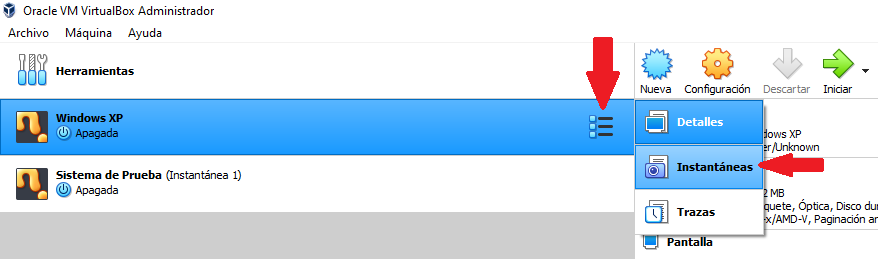
\includegraphics[scale = 0.5]{img/instantanea1.png}
        \caption{Seleccionamos la pestaña Instantánea.}
        \label{Instantanea1}
      \end{figure}

      \newpage

      Seguidamente seleccionamos la opción: \textbf{"Tomar"} o podemos usar el atajo \texttt{CTRL + SHIFT + T}, tal como se muestra en la captura.
      \begin{figure}[h]
        \centering
        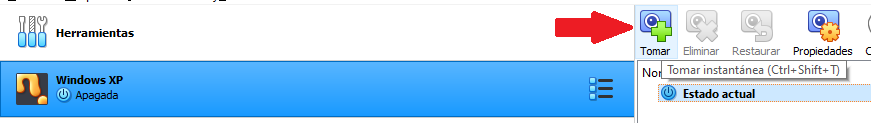
\includegraphics[scale = 0.5]{img/instantanea2.png}
        \caption{Realizamos la instantánea.}
        \label{Instantanea2}
      \end{figure}
      \\
      Nos aparecerá una ventana donde incluiremos el nombre de la Instantánea y una descripción para tenerlo todo ordenado y bien localizable.
      \begin{figure}[h]
        \centering
        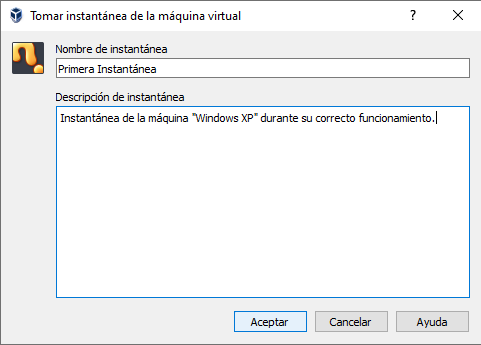
\includegraphics[scale = 1]{img/instantanea3.png}
        \caption{Descripción de la instantánea.}
      \end{figure}
      \label{Instantanea3}
      \\
      Ahora, después de realizar todos los pasos, deberíamos ver algo así en nuestro sistema de virtualización.
      \begin{figure}[h]
        \centering
        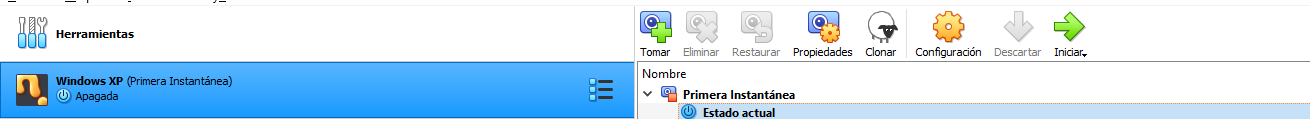
\includegraphics[scale = 0.5]{img/instantanea4.png}
        \caption{Resultado final de la captura de instantáneas.}
        \label{Instantanea4}
      \end{figure}

      \newpage

      *inserte operación destructiva*

      \newpage
    
    \section{Clonado}
      En este apartado \textit{realizaremos un clonado de un sistema invitado en un disco independiente comprobando que 
      podemos ejecutar los dos sistemas simultaneamente.}
      \\
      Para realizar el clonado de una máquina nos iremos al mismo menú de \textbf{la figura }\ref{Instantanea1}.
      y pulsamos en el boton de \textbf{Clonar}, nos aparecerá una ventana con las opciones que tenemos que seleccionar 
      para la realización del clonado.
      \begin{figure}[h]
        \centering
        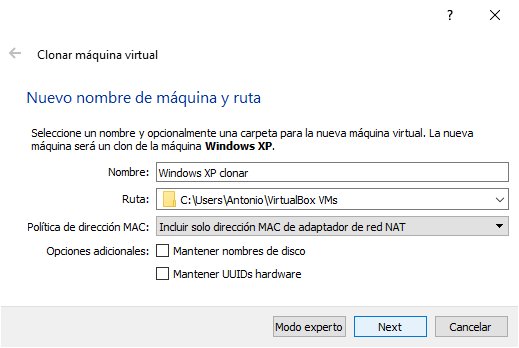
\includegraphics[scale = 0.75]{img/clonar1.png}
        \caption{Opciones para el clonado.}
        \label{Clonado1}
      \end{figure}
      Debemos nombrar a la maquina clonada, la ruta donde se guardaría la máquina, la política de la dirección MAC, y unas 
      operaciones adicionales y pulsamos \textit{"next"}.
      \begin{figure}[h]
        \centering
        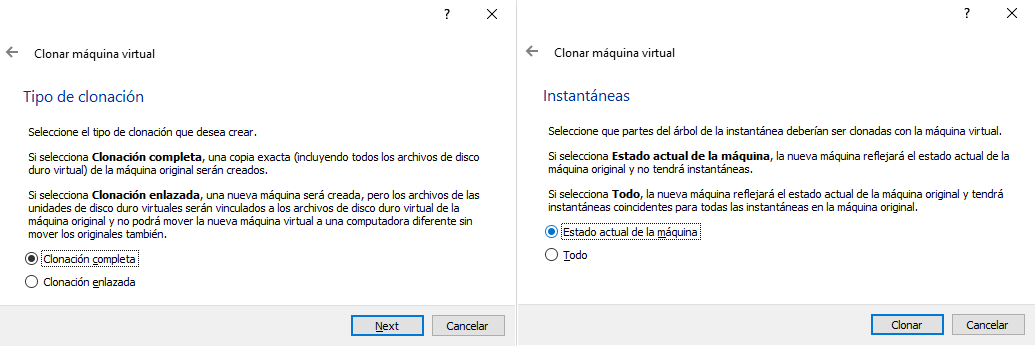
\includegraphics[scale = 0.5]{img/clonar2.png}
        \caption{Diferentes ventanas para el clonado.}
        \label{Clonado2}
      \end{figure}
      Seguidamente nos aparecerá un par de ventanas donde tenemos que elegir si clonar la máquina enlazadamente o una clonación 
      completa e incluso el monmento de clonación de la máquina, si el actual o algún otro.

      \newpage

      En el siguiente paso de este apartado debemos ejecutar a la vez las dos máquinas que hemos creado, \textit{Windows XP y Windows XP clonar}.
      \begin{figure}[h]
        \centering
        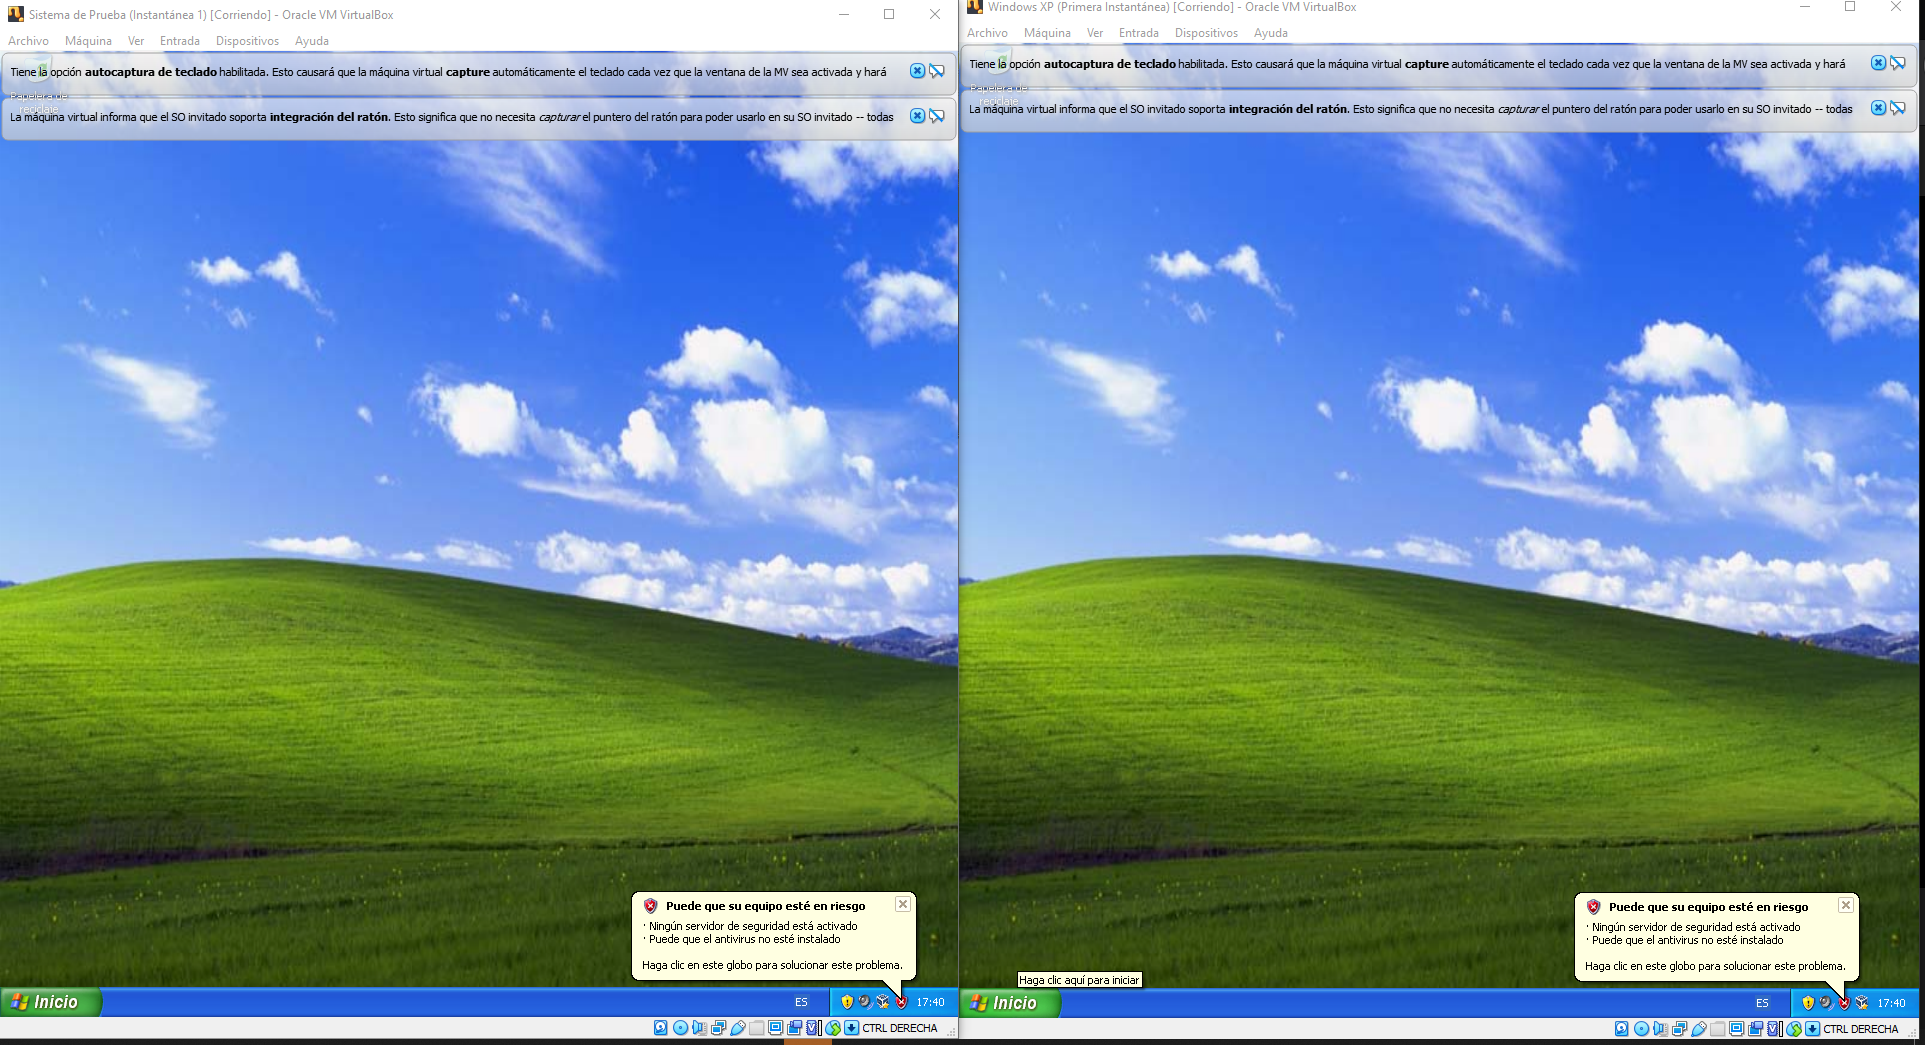
\includegraphics[scale = 0.3]{img/clonar3.png}
        \caption{Dos máquinas corriendo a la vez.}
        \label{Clonado3}
      \end{figure}
      \\
      Vemos que efectivamente, el posible correr las dos máquinas virtuales a la vez.

      \newpage

    \section{Configuración de red modo NAT}
      En este apartado comprobaremos el direccionamiento y la conectividad desde el sistema invitado al anfitrión y viceversa.
      \\\\
      En primer lugar debemos comprobar que el protocolo de la tarjeta de red de nuestra máquina es el adecuado, en el caso de 
      este apartado el modo \textbf{NAT}. Lo haremos pulsando en el botón de red y comprobamos que esté puesto el modo \textbf{NAT}.
      \\
      \begin{figure}[h]
        \centering
        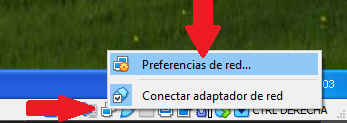
\includegraphics{img/clonar4.png}
        \caption{Botón de red.}
        \label{Nat1}
      \end{figure}
      \\
      \begin{figure}[h]
        \centering
        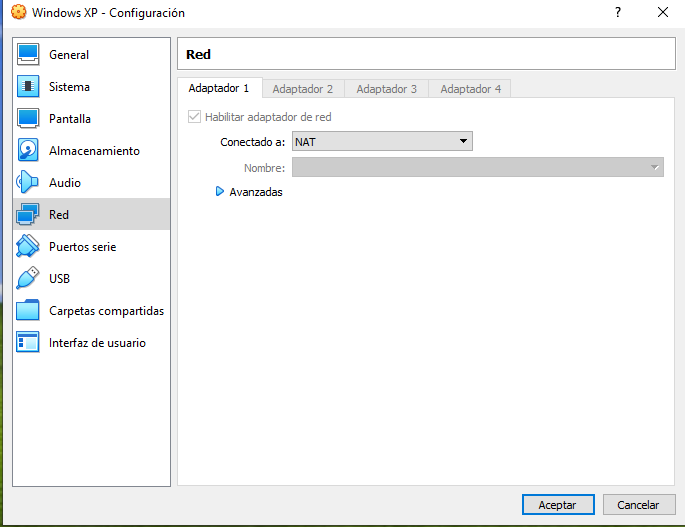
\includegraphics[scale = 0.5]{img/clonar5.png}
        \caption{Opción de red.}
        \label{Nat2}
      \end{figure}

      \newpage

      La dirección de nuestra máquina invitada es: \texttt{10.0.2.15} y la dirección de nuestra máquina anfitrión es: \texttt{192.168.1.35}, 
      para conprobar el direccionamiento debejemos ejecutar el comando \texttt{ping} desde la máquina que deseemos junto con la ruta de la 
      máquina a la que queremos comprobar el direccionamiento.
      \\
      Primeramente desde la máquina anfitrión comprobamos el direccionamiento hacia la máquina invitada, haciendo uso de lo comentado anteriormente.
      El resultado sería el siguiente:
      \\
      \begin{figure}[h]
        \centering
        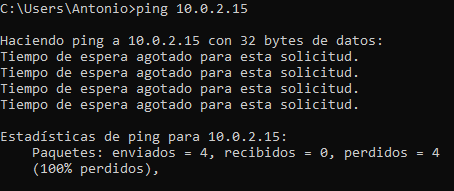
\includegraphics{img/nat1.png}
        \caption{Resultado del ping a máquina invitada.}
        \label{Nat3}
      \end{figure}
      \\
      Podemos comprobar que el direccionamiento de red desde la máquina anfitrión a la máquina invitada no está funcionando.
      \\\\
      Seguidamente, comprobamos la operación viceversa.
      \begin{figure}[h]
        \centering
        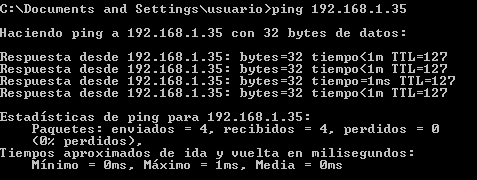
\includegraphics{img/nat2.png}
        \caption{Resultado del ping a máquina anfitrión.}
        \label{Nat4}
      \end{figure}
      \\
      En esto caso podemos comprobar que funciona perfectamente.

      \newpage

    \section{Configuración de red modo BRIDGE(puente)}
      En este apartado debemos comprobar el direccionamiento y la conectividad desde el sistema invitado al anfitrión y viceversa.


\end{document}